\chapter{Applications}

\fbox{
    \parbox{\textwidth}
    {
        Chapter Overview
        \begin{itemize}
            \item Empirical analysis of BayesCNN with normal architecture for Image Super Resolution.
            \item Empirical analysis of BayesCNN with normal architecture for Generative Adversarial Networks.
        \end{itemize}
    }
}

\pagebreak



\section{BayesCNN for Image Super Resolution}

The task referred as Super Resolution is the recovery of a High Resolution image from a given Low Resolution image. It is applicable to many areas like medical imaging \citet{10.1007/978-3-642-40760-4_2}, face recognition \citet{1203152} and so on.

There are many ways to do a single image super resolution and a detailed benchmarks of the methods is provided by Yang \citet{Yang2014SingleImageSA}. Following are the major ways to do a single image super resolution:\\ 

\textbf{Prediction Models}: These models generate High Resolution images
from Low Resolution inputs through a predefined mathematical formula. No training data is needed for such models. Interpolation-based methods (bilinear, bicubic, and Lanczos) generate HR pixel intensities by weighted averaging neighboring LR pixel values are good examples of this method.\\

\textbf{Edge Based Methods}: Edges are one of the most important features for any computer vision task. The High Resolution Images learned from the edge features high quality edges and good sharpness. However these models lack good color and textures information.\\

\textbf{Patch Based Methods}: Cropped patches from Low Resolution Images aand High Resolution Images are taken from training dataset to learn some mapping function. The overlapped patches are averaged or some other techniques like Conditional Random Fields \citet{lafferty2001conditional} can be used for better mapping of the patches.  


\subsection{Our Approach}

We build our work upon \citet{DBLP:journals/corr/ShiCHTABRW16} work that shows that performing Super Resolution work in High Resolution space is not the optimal solution and it adds the computation complexity. We used a Bayesian Convolutional Neural Network to extract features in the Low Resolution space. We use an efficient sub-pixel convolution layer, as proposed by \citet{DBLP:journals/corr/ShiCHTABRW16}, which learns an array of upscaling filters to upscale the final Low Resolution feature maps into the High Resolution output. This replaces the handcrafted bicubic filter in the Super Resolution pipeline with more complex upscaling filters specifically trained for each feature map, and also reduces the computational complexity of the overall Super Resolution operation.

\begin{figure*}[htbp]
\begin{center}
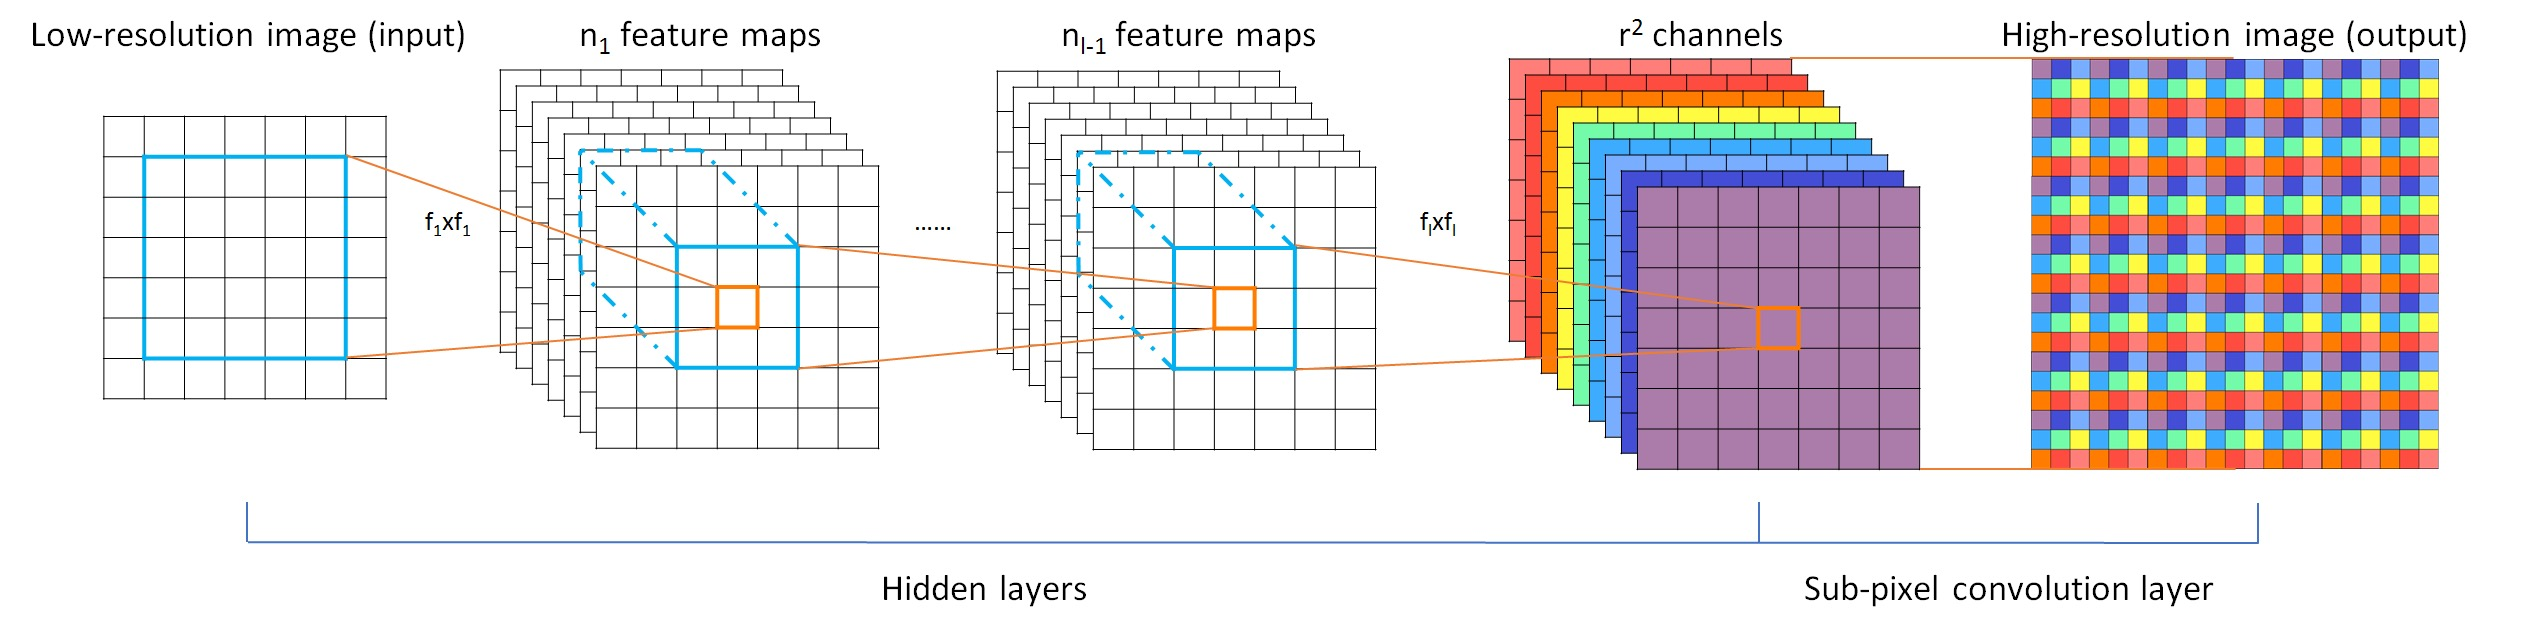
\includegraphics[width=1.0\linewidth]{Chapter6/Figs/networkstructure.jpg}
\caption{The proposed efficient sub-pixel convolutional neural network (ESPCN) \cite{DBLP:journals/corr/ShiCHTABRW16}, with two convolution layers for feature maps extraction, and a sub-pixel convolution layer that aggregates the feature maps from Low Resolution space and builds the Super Resolution image in a single step.}
\label{fig:networkstructure}
\end{center}
\end{figure*}

We used a four layer convolutional model as mentioned in the paper \cite{DBLP:journals/corr/ShiCHTABRW16}. We replaced the convolution layer by Bayesian convolution layer and changed the forward pass that now computes the mean, variance and KL divergence. The PixelShuffle layer is kept same as provided by PyTorch and no changes has been made there.  

\begin{table}[H]
    \centering
    \renewcommand{\arraystretch}{2}
    \begin{tabular}{c c c c } 
 \hline
 layer type & width & stride & padding  \\ [0.5ex] 
 \hline
 convolution ($5\times5$) & 64 & 1 & 2 \\
 
 convolution ($3\times3$) & 64 & 1 & 1 \\
 
 
 convolution ($3\times3$) & 32 & 1 & 1 \\
 
 convolution ($3\times3$) & upscale factor * * 2 & 1 & 1  \\ [1ex] 
 \hline
\end{tabular}
\renewcommand{\arraystretch}{1.5}
\label{tab:SuperResolutionArchitecture}
\caption{Network Architecture for Bayesian Super Resolution}
\end{table}

Where \textit{upscale factor} is defined as a parameter. For our experiments, we take upscale factor = 3. 

\subsection{Empirical Analysis}

The Network architecture was trained on BSD300 dataset \cite{MartinFTM01} provided by the Berkeley Computer Vision Department. The dataset is very popular for Image Super Resolution task and thus the dataset is used to compare the results with other work in the domain. 

\begin{figure}[H]
\begin{center}
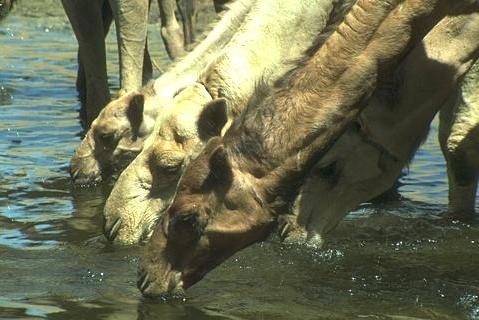
\includegraphics[height=.28\textheight]{Chapter6/Figs/camel_LR.png}
\label{fig:CamelLR}
\caption{Sample image in Low Resolution image space taken randomly from BSD 300 \cite{MartinFTM01} dataset.}
\end{center}
\end{figure}

\begin{figure}[H]
\begin{center}
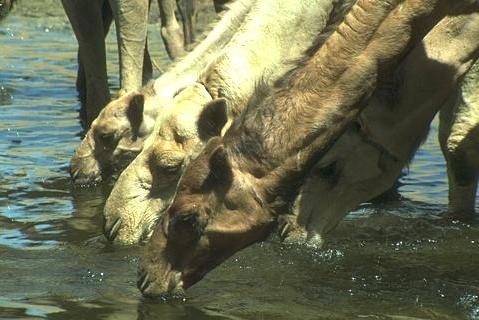
\includegraphics{Chapter6/Figs/camel_LR.png}
\label{fig:CamelSR}
\caption{Generated Super Resolution Image}
\end{center}
\end{figure}




\section{BayesCNN for Generative Adversarial Networks}

Generative Adversarial Networks (GANs) \cite{goodfellow2014generative} can be used for two major tasks: to learn good feature representations by using the generator and discriminator networks as feature extractors, and to generate natural images. The learned feature representation or generated images can reduce the number of images substantially for a computer vision supervised task. However GANs were quite unstable to train in the past and that is why we base our work on the stable GAN architecture namely Deep Convolutional GANs (DCGAN) \cite{DBLP:journals/corr/RadfordMC15}. We use the trained Bayesian discriminators for image classification tasks, showing competitive performance with the normal DCGAN architecture.



\subsection{Our approach}
\subsection{Empirical Analysis}



